\chapter{Accurate Newton's Method for B\'{e}zier Curve Intersection}
\label{chap:compensated-newton}

\section{Introduction}

When using Newton's method to find the root of a function via
\begin{equation}
G\left(\bm{x}\right) = \bm{x} - J^{-1} F\left(\bm{x}\right)
\end{equation}
there are three computations performed that can introduce instability:
evaluation of the residual function \(F\left(\bm{x}\right)\), evaluation
of the Jacobian \(J\) and solution of the linear system \(J \bm{y} =
F\left(\bm{x}\right)\). In \cite{Tisseur2001}, the author showed that by
just using a more precise evaluation of the residual function, the
accuracy of Newton's method can be improved.

This chapter considers Newton's method applied to two problems:
root-finding for polynomials expressed in Bernstein form and
intersection of two B\'{e}zier curves in \(\reals^2\). In both problems,
the compensated de Casteljau method (see Chapter~\ref{chap:k-compensated}) is
used for evaluation of the residual. When evaluating a polynomial
\(p(s)\) this is straightforward, but when evaluating the difference
\(b_1(s) - b_2(t)\) between two curves special care must be taken.

\begin{figure}
  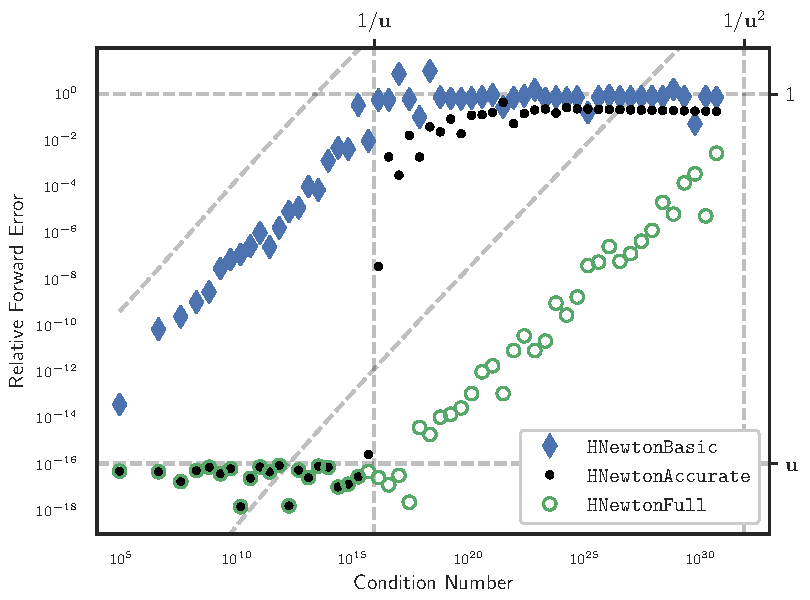
\includegraphics{../images/compensated-newton/newton_jghplus13.pdf}
  \centering
  \captionsetup{width=.75\linewidth}
  \caption{Comparing relative error to condition number when using Newton's
    method to find a root of \(p(s) = (s - 1)^n - 2^{-31}\), where polynomial
    evaluation occurs via Horner's method.}
  \label{fig:jgh+13}
\end{figure}

In \cite{Graillat2008}, the problem of finding simple roots \(\alpha\) of
polynomials \(p(s)\) expressed in the monomial basis is considered.
A standard Newton's method (\texttt{HNewtonBasic}) that evaluates \(p(s)\)
and \(p'(s)\) using Horner's method is compared to a modified Newton's method
(\texttt{HNewtonAccurate}) that evaluates \(p(s)\) with a compensated
Horner's method. This proceeds as in \cite{Tisseur2001}: the evaluation of
the residual is done with greater accuracy but the rest of the process
is the same. When computing a root \(\alpha\), the standard Newton's method
has a relative error that grows linearly with the condition number of the
root (which will be defined in Section~\ref{sec:conditioning}). The
modified Newton's method is fully accurate to machine precision (i.e.
the relative error is \(\bigO{\mach}\)) until \(\cond{\alpha}\) reaches
\(1/\mach\), as seen in Figure~\ref{fig:jgh+13}.

After the point where \texttt{HNewtonAccurate} loses accuracy, we'd
expect a linear increase in relative error based on a compensated
rule of thumb:
\begin{equation}
\frac{\left|\widehat{\alpha} - \alpha\right|}{\left|\alpha\right|} \leq
  c_1 \mach + c_2 \cond{\alpha} \mach^2
\end{equation}
where \(c_1 \mach\) corresponds to rounding into the given
precision and \(c_2 \cond{\alpha} \mach^2\) reflects the
typical error but from computations done with working precision
\(\overline{\mach} = \mach^2\). The point
where the condition number exceeds \(1/\mach\) should correspond to
the point where the second term is larger that the
first term. However, this is not possible unless the
Jacobian (i.e. \(p'(s)\)) is also evaluated with a compensated
method. A second modified Newton's method (\texttt{HNewtonFull}) is
introduced in \cite[Section~8]{Jiang2013} and the author shows that
this second modified Newton's method does indeed follow a compensated
rule of thumb under appropriate conditions. We see in
Figure~\ref{fig:jgh+13} that \texttt{HNewtonFull} enables
\(\bigO{\mach}\) relative errors until the condition number reaches
\(1/\mach\) and then a linear increase in error as the condition number
grows from \(1/\mach\) to \(1/\mach^2\).

We'll proceed similarly for polynomials in
Bernstein form. Since this is a one dimensional Newton's method, improving
the evaluation of the Jacobian is straightforward. The results agree with
what has been observed when using Horner's method for evaluation.

Computing the intersection(s) of two parametric plane curves is a
common task in computational geometry and has many uses, e.g. in
finite element methods that use overlapping curved meshes. Many
methods have been described in the literature to solve this problem.
Algebraic methods such as implicitization and eigenvalue-based
methods (e.g. \cite{Manocha:CSD-92-698}) suffer
from accuracy issues for moderately high degrees and can often be
very complex to implement. Some (\cite{Bates2008}) even rely on symbolic
algebraic manipulations, which can be quite costly since it requires
arbitrary precision.
Geometric methods (e.g. \cite{Sederberg1986, Sederberg1990, Kim1998})
typically use a form of domain splitting to focus on subproblems and
eliminate parts of the domain where an intersection is guaranteed not
to occur. After a domain has been sufficiently reduced, Newton's method
is used for the last few bits of accuracy.

We'll focus on transversal curve intersections that are ill-conditioned.
Transversal intersections are an extension of the concept of a
simple root. A non-transversal intersection occurs when the curves
or tangent at the point of intersection or when one of the curves
has a zero tangent vector at that point, either due to an improper
parameterization (e.g. \(x(s) = s^2, y(s) = s^2 + 1\)) or a cusp.
In many cases, transversal intersections that are ``almost tangent'' have
very high condition numbers.

The chapter is organized as follows. In Section~\ref{sec:conditioning}
we define and discuss the conditioning of both a simple root and
a transversal intersection. In Section~\ref{sec:compensated-simple-roots}
we describe two compensated Newton's methods for finding simple roots
and perform a numerical experiment verifying the expected behavior.
In Section~\ref{sec:compensated-curve-intersect} we describe a
compensated Newton's method for B\'{e}zier curve intersection and
perform sever numerical experiements to verify the expected behavior
on both transversal intersections and tangent intersections (i.e.
intersections with infinite condition number).
Section~\ref{sec:false-starts} acts as a
coda: it describes some failed attempts at constructing numerical
examples. This section provides an in-depth discussion of a particular
family of polynomials that has much better than expected conditioning
when written in the Bernstein basis.

\section{Problem conditioning}\label{sec:conditioning}

Consider a smooth function \(F: \reals^n \longrightarrow \reals^n\)
with Jacobian \(F_{\bm{x}} = J\). We want to consider a special class of
functions of the form \(F\left(\bm{x}\right) = \sum_j c_j
\phi_j\left(\bm{x}\right)\) where the basis
functions \(\phi_j\) are also smooth functions on \(\reals^n\)
and each \(c_j \in \reals\). We want to consider the effects on a root
\(\bm{\alpha} \in \reals^n\) of a perturbation in one of the
coefficients \(c_j\). We examine the perturbed functions
\begin{equation}
G(x, \delta) = F\left(\bm{x}\right) + \delta \phi_j\left(\bm{x}\right).
\end{equation}
Since \(G\left(\bm{\alpha}, 0\right) = \bm{0}\), if \(J^{-1}\) exists at
\(\bm{x} = \bm{\alpha}\) then
the implicit function theorem tells us that we can define
\(\bm{x}\) via
\begin{equation}
G\left(\bm{x}\left(\delta\right), \delta\right) = \bm{0}.
\end{equation}
Taking the derivative with respect to \(\delta\) we find that
\(\bm{0} = G_{\bm{x}} \bm{x}_{\delta} + G_{\delta}\). Plugging in
\(\delta = 0\) we find that \(0 = J\left(\bm{\alpha}\right) \bm{x}_{\delta} +
\phi_j\left(\bm{\alpha}\right)\), hence we
conclude that
\begin{equation}
\bm{x}\left(\delta\right) = \bm{\alpha} - J\left(\bm{\alpha}\right)^{-1}
  \phi_j\left(\bm{\alpha}\right) \delta + \bigO{\delta^2}.
\end{equation}
This gives a relative condition number (for the root) of
\begin{equation}
\frac{\left \lVert J\left(\bm{\alpha}\right)^{-1}
  \phi_j\left(\bm{\alpha}\right) \right \rVert}{
  \left \lVert \bm{\alpha} \right \rVert}.
\end{equation}

By considering perturbations in \textbf{all} of the coefficients:
\(\left|\delta_j\right| \leq \eps \left|c_j\right|\), a similar analysis
gives a root function
\begin{equation}
\bm{x}\left(\delta_0, \ldots, \delta_n\right) = \bm{\alpha} -
  J\left(\bm{\alpha}\right)^{-1} \sum_{j = 0}^n \delta_j
  \phi_j\left(\bm{\alpha}\right) + \bigO{\eps^2}.
\end{equation}
With this, we can define a root condition number
\begin{equation}\label{eq:abstract-cond-num}
\kappa_{\bm{\alpha}} =
  \lim_{\eps \to 0} \left(\sup \frac{\left \lVert\delta \bm{\alpha}
  \right \rVert / \eps}{\left \lVert\bm{\alpha}\right \rVert}\right) =
  \lim_{\eps \to 0} \left(\sup \frac{\left \lVert
  J\left(\bm{\alpha}\right)^{-1} \sum_j \delta_j
  \phi_j\left(\bm{\alpha}\right) \right \rVert / \eps}{
  \left \lVert\bm{\alpha}\right \rVert}\right).
\end{equation}

When \(n = 1\), \(J^{-1}\) is simply \(1 / F'\) and we find
\begin{equation}
\kappa_{\alpha} =
  \frac{1}{\left|\alpha F'(\alpha)\right|} \sum_{j = 0}^n \left|
  c_j \phi_j(\alpha)\right|.
\end{equation}
This value is given by the triangle inequality applied to
\(\delta \alpha\)  and equality can be attained since the sign
of each \(\delta_j = \pm c_j \eps\) can be modified at will to make
\(\phi_j(\alpha) \delta_j = \left|\phi_j(\alpha) c_j\right| \eps\).

When \(n > 1\), the triangle inequality tells us that
\begin{equation}
\kappa_{\bm{\alpha}} =
  \lim_{\eps \to 0} \left(\sup \frac{\left \lVert\delta \bm{\alpha} /
  \eps\right \rVert}{\left \lVert\bm{\alpha}\right \rVert}\right) \leq
  \frac{1}{\left \lVert\bm{\alpha}\right \rVert} \sum_{j = 0}^n
  \left|c_j\right| \left \lVert J\left(\bm{\alpha}\right)^{-1}
  \phi_j(\bm{\alpha})\right \rVert.
\end{equation}
However, this bound is only attainable if all
\(\phi_j(\bm{\alpha})\) are parallel. However, we'll seldom need to
compute the exact condition number and are instead typically
interested in the order of magnitude. In this case a lower
bound
\begin{equation}
\frac{1}{\left \lVert\bm{\alpha}\right \rVert}
\max_j \left|c_j\right| \left \lVert J\left(\bm{\alpha}\right)^{-1}
\phi_j(\bm{\alpha})\right \rVert
\end{equation}
for \(\kappa_{\bm{\alpha}}\)
will suffice as an approximate condition number.

For an example, consider
\begin{equation}
\phi_0 = \left[ \begin{array}{c} x_0 \\ 2 \\ 0 \end{array}\right],
\phi_1 = \left[ \begin{array}{c} 0 \\ x_1 \\ 3 \end{array}\right],
\phi_2 = \left[ \begin{array}{c} 2 \\ 0 \\ x_2 \end{array}\right],
F = \phi_0 + 2 \phi_1 + 3 \phi_2,
\bm{\alpha} = \left[ \begin{array}{c} -6 \\ -1 \\ -2 \end{array}\right].
\end{equation}
For a given \(\eps\), the maximum root perturbation occurs when
\(\delta_0 = \eps, \delta_1 = 2 \eps, \delta_2 = -3 \eps\) and
gives
\(\left \lVert J\left(\bm{\alpha}\right)^{-1} \sum_j
\delta_j \phi_j\left(\bm{\alpha}\right) \right \rVert
= 4 \sqrt{10} \eps \approx 12.65 \eps\).
The pessimistic triangle inequality bound gives
\(\sum_j \left|c_j\right| \left \lVert J\left(\bm{\alpha}\right)^{-1}
\phi_j(\bm{\alpha})\right \rVert \approx 14.64 \eps\) and the
maximum individual perturbation is \(2 \sqrt{10} \eps \approx 6.325 \eps\)
(this occurs when \(\delta_0 = \delta_1 = 0, \delta_2 = \pm 3 \eps\)).

In this general framework, we can define a condition number both
for a simple root of a polynomial in Bernstein form and for the
intersection of two planar B\'{e}zier curves. For the first,
\(\phi_j(s) = \binom{n}{j} (1 - s)^{n - j} s^j\) the Bernstein basis
functions, a polynomial \(p(s) = \sum_j b_j \phi_j(s)\) with
a simple root \(\alpha \in \left(0, 1\right]\) has root condition number
\begin{equation}
\kappa_{\alpha} =
  \frac{1}{\alpha \left|p'(\alpha)\right|} \sum_{j = 0}^n \left|
  b_j \phi_j(\alpha)\right| = \frac{\widetilde{p}(\alpha)}{
  \alpha \left|p'(\alpha)\right|}.
\end{equation}
For the intersection of a degree \(m\) curve \(b_1(s)\) and
a degree \(n\) curve \(b_2(t)\), we have basis functions
\begin{multline}
\phi_{0, -1, 1} = \left[ \begin{array}{c} B_{0, m}(s) \\ 0 \end{array}\right],
\phi_{0, -1, 2} = \left[ \begin{array}{c} 0 \\ B_{0, m}(s) \end{array}\right],
\cdots, \\
\phi_{m, -1, 1} = \left[ \begin{array}{c} B_{m, m}(s) \\ 0 \end{array}\right],
\phi_{m, -1, 2} = \left[ \begin{array}{c} 0 \\
  B_{m, m}(s) \end{array}\right], \\
\phi_{-1, 0, 1} = \left[ \begin{array}{c} -B_{0, n}(t) \\
  0 \end{array}\right],
\phi_{-1, 0, 2} = \left[ \begin{array}{c} 0 \\
  -B_{0, n}(t) \end{array}\right], \cdots, \\
\phi_{-1, n, 1} = \left[ \begin{array}{c} -B_{n, n}(t) \\
  0 \end{array}\right], \phi_{-1, n, 2} = \left[ \begin{array}{c} 0 \\
  -B_{n, n}(t) \end{array}\right].
\end{multline}
Since \(F(s, t) = b_1(s) - b_2(t)\) we have Jacobian \(J(s, t) =
\left[ \begin{array}{c c} b_1'(s) & -b_2'(t) \end{array}\right]\). We'll
consider a transversal intersection \(F(\alpha, \beta) = \bm{0}\) with
\(\det J(\alpha, \beta) \neq 0\). Since each of the
\(\phi_j\) is just a scalar multiple of the standard basis
vectors, writing \(J^{-1} = \left[ \begin{array}{c c}
\bm{v}_1 & \bm{v}_2 \end{array}\right]\), we have
\begin{multline}
J\left(\alpha, \beta\right)^{-1} \sum_{\bm{j}} \delta_{\bm{j}}
  \phi_{\bm{j}}\left(\alpha, \beta\right) = \left[\sum_{i = 0}^m
  \delta_{i, -1, 1} B_{i, m}\left(\alpha\right) + \sum_{j = 0}^n
  \delta_{-1, j, 1} B_{j, n}\left(\beta\right)\right] \bm{v}_1 \\
+ \left[\sum_{i = 0}^m
  \delta_{i, -1, 2} B_{i, m}\left(\alpha\right) + \sum_{j = 0}^n
  \delta_{-1, j, 2} B_{j, n}\left(\beta\right)\right] \bm{v}_2 =
  \nu_1 \bm{v}_1 + \nu_2 \bm{v}_2.
\end{multline}
where
\begin{equation}\label{eq:nu-bounds}
\left|\nu_k\right| / \eps \leq \sum_{i = 0}^m
  \left|c_{i, -1, k}\right| B_{i, m}\left(\alpha\right) + \sum_{j = 0}^n
  \left|c_{-1, j, k}\right| B_{j, n}\left(\beta\right) = \mu_k
\end{equation}
and the bound can be attained for both \(k = 1, 2\) by making the
signs of the \(\delta_{\bm{j}}\) agree. If we name the components of each
curve via
\(b_1(s) = \left[ \begin{array}{c c} x_1(s) & y_1(s) \end{array}\right]^T\)
and \(b_2(t) = \left[ \begin{array}{c c} x_2(t) & y_2(t) \end{array}\right]^T\)
then we see that \(\mu_1 = \widetilde{x}_1(\alpha) + \widetilde{x}_2(\beta)\)
and \(\mu_2 = \widetilde{y}_1(\alpha) + \widetilde{y}_2(\beta)\).
Thus we have condition number
\begin{align}
\kappa_{\alpha, \beta} &= \frac{1}{\sqrt{\alpha^2 + \beta^2}}
  \max_{\left|\nu_k\right| \leq \mu_k} \left \lVert \nu_1 \bm{v}_1 +
  \nu_2 \bm{v}_2 \right \rVert_2 \\
  &=
  \sqrt{\frac{\max_{\left|\nu_k\right| \leq \mu_k}
  \nu_1^2 \left(\bm{v}_1 \cdot \bm{v}_1\right) +
  2 \nu_1 \nu_2 \left(\bm{v}_1 \cdot \bm{v}_2\right) +
  \nu_2^2 \left(\bm{v}_2 \cdot \bm{v}_2\right)}{\alpha^2 + \beta^2}}
  \label{eq:intersect-cond-num}.
\end{align}
Since \(J^{-1}\) is invertible, we know \(\bm{v}_1\) and \(\bm{v}_2\) are
not parallel which can be used to show that the only internal critical
point of the function to be maximimized in~\eqref{eq:intersect-cond-num}
is \(\nu_1 = \nu_2 = 0\), which is the global minimum. Along the boundary of
the rectangle
\(\left[-\mu_1, \mu_1\right] \times \left[-\mu_2, \mu_2\right]\),
we fix one of \(\nu_1\) or \(\nu_2\) and the resulting univariate function is
an up-opening parabola, hence any critical point must be a local
minimum. Thus we know the maximum occurs at two of the four corners of the
rectangle:
\begin{equation}\label{eq:intersect-cond-num-too}
\kappa_{\alpha, \beta} = \sqrt{\frac{\mu_1^2
  \left(\bm{v}_1 \cdot \bm{v}_1\right) +
  2 \mu_1 \mu_2 \left|\bm{v}_1 \cdot \bm{v}_2\right| +
  \mu_2^2 \left(\bm{v}_2 \cdot \bm{v}_2\right)}{\alpha^2 + \beta^2}}.
\end{equation}

As far as the author can tell,
a condition number for the intersection of two planar B\'{e}zier curves
has not been described in the Computer Aided Geometric Design (CAGD)
literature. In \cite[Chapter~25, Equation 25.11]{Higham2002}
a more generic condition number is defined for the root of a nonlinear
algebraic system that is similar to the definition above.

For an example, consider the line
\(b_1(s) = \left[ \begin{array}{c c} 2s & 2s \end{array}\right]^T\)
and improperly parameterized line
\(b_2(t) = \left[ \begin{array}{c c} 4t^2 & 2 - 4t^2
\end{array}\right]^T\) which intersect at \(\alpha = \beta = 1/2\).
At the intersection we have \(J^{-1} = \frac{1}{8}
\left[ \begin{array}{c c} 2 & 2 \\ -1 & 1 \end{array}\right]\),
so that \(\bm{v}_1 \cdot \bm{v}_1 = \bm{v}_2 \cdot \bm{v}_2 =
5/64\) and \(\bm{v}_1 \cdot \bm{v}_2 = 3/64\). Since the
\(x\)-component of \(F(s, t)\) can be written as
\(2s - 4t^2 = 2 B_{1, 1}(s) - 4 B_{2, 2}(t)\) and the
\(y\)-component as \(2s + 4t^2 - 2 = 2 B_{1, 1}(s) - 2 B_{0, 2}(t)
- 2 B_{1, 2}(t) + 2 B_{2, 2}(t)\) we have
\begin{alignat}{2}
\mu_1 &= 2 B_{1, 1}(\alpha) &&+ 4 B_{2, 2}(\beta) = 2 \\
\mu_2 &= 2 B_{1, 1}(\alpha) + 2 B_{0, 2}(\beta) +
  2 B_{1, 2}(\beta) &&+ 2 B_{2, 2}(\beta) = 3.
\end{alignat}
Following~\eqref{eq:intersect-cond-num-too}, this gives
\(\kappa_{\alpha, \beta} = \sqrt{202}/8 \approx 1.78\).

\section{Simple polynomial roots}\label{sec:compensated-simple-roots}

Placeholder.

\section{B\'{e}zier curve intersection}\label{sec:compensated-curve-intersect}

Placeholder.

\section{False starts}\label{sec:false-starts}

It was quite challenging to generate families of polynomials with known
ill-conditioned simple roots and families of B\'{e}zier curve pairs with known
ill-conditioned transversal intersections. The issue was not in finding a
family with moderately high condition number, but in finding one where the
condition number would grow past \(1 / \mach\) and even as far as
\(1 / \mach^2\). In many failed attempts, as the condition increased
in a given family, it became impossible to represent the
coefficients exactly in \(\floats\). Once the coefficients are rounded,
the roots or intertesections themselves will likely move erratically.
This erratic behavior is the goal when generating ill-conditioned problems,
but makes the values themselves less useful.

To give a sense of the nontrivial effort involved in finding a
family, consider the following families of polynomials that
\textbf{failed}:
\begin{itemize}
  \itemsep 0em
  \item \(p(s) = (1 - s)^n - 2^{-d}\) at the simple root
    \(s_{\ast} = 1 - 2^{-d/n}\). In the monomial basis, the
    condition number of \(s_{\ast}\) grows exponentially and was used
    as the example in \cite{Graillat2008} and \cite[Section~8]{Jiang2013}.
    However in the Bernstein basis, the root condition
    number is always less than \(1\).
  \item \(p(s) = (as - 1)^n - 2^{-d} (1 - s)^n\) at the simple root
    \(s_{\ast} = \frac{1 + 2^{-d/n}}{a + 2^{-d/n}}\). This is problematic
    because when \(a - 1\) is not a power of \(2\), the coefficients
    in \((as - 1)^n = \left[-(1 - s) + (a - 1)s\right]^n\) cannot be
    represented exactly in \(\floats\) for high enough degree. The rounded
    coefficients result in sporadic behavior for the resulting polynomials.
    When \(a - 1 = 2^d\), Newton's method converges with much better than
    expected accuracy due to a unique quirk of the de Casteljau algorithm.
    This case is interesting enough to consider in greater detail
    in \cite{Hermes2018}.
  \item \(p(s) = (2s - 1)^n - 2^{-52}\) at the simple root
    \(s_{\ast} = \frac{1 + 2^{-52/n}}{2}\). The coefficients \(b_j =
    (-1)^{n - j} - 2^{-52}\) can always be represented in \(\floats\),
    but as \(n \to \infty\) we have \(s_{\ast} \to 1\).
    A root exactly equal to \(1\) is perfectly conditioned, so
    unsurprisingly \(\kappa \to 0\) after reaching a maximum
    value of \(\approx 3 \cdot 10^{13}\) when \(n = 28\).
  \item \(p(s) = (3s - 1)^n - 2^{-d}\) at the simple root \(s_{\ast} = \frac{
    1 + 2^{-d/n}}{3}\). The coefficients \(b_j = (-1)^{n - j} 2^j - 2^{-d}\)
    can be represented exactly in \(\floats\) for \(\left|j + d\right|
    \leq 52\) (or \(53\), depending on \(n\)). This limitation stops the
    condition number from growing large enough. For example, when \(d = 10\),
    the largest term that can be represented exactly is \(\kappa_{43}
    \approx 1.03 \cdot 10^{10}\),
    when \(d = 20\), the largest term that
    can be represented exactly is \(\kappa_{33} \approx 2.53 \cdot 10^{10}\)
    and when \(d = 30\), the largest term that
    can be represented exactly is \(\kappa_{23} \approx 9.24 \cdot 10^{10}\).
\end{itemize}

In addition, several false starts were made when generating a family of
B\'{e}zier curve pairs with ill-conditioned intersection. In the
case of polynomials we increased the condition number via the degree,
but in the case of curve pairs it was increased by reducing a continuous
parameter towards zero at which point the pair becomes tangent. The
most problematic case came from
\begin{equation}
F(s, t; r) = \left[ \begin{array}{c} 2(4s^2 - 1) + r \\ (2s - 1)^2
\end{array}\right] - \left[ \begin{array}{c} 4(4t^2 - 1) \\ 4(2t - 1)^2
\end{array}\right].
\end{equation}
In this case, the polynomials \((2s - 1)^2\) and \(4(2t - 1)^2\) come
from a very special class of polynomials described in \cite{Hermes2018}
where the de Casteljau algorithm is very accurate (much better than
the a priori upper bound). As a result, the \(y\)-contributions to the
relative error were essentially zero. This can be thought of as setting
\(\mu_2 = 0\) when computing the condition number. However, for this family
of curves the \(x\)-components contribute \(\bigO{1}\) to the condition
number while the \(y\)-components \textit{should} contribute \(\bigO{1/r}\)
but instead contribution nothing. Hence the solution can always be computed
by Newton's method with \(\bigO{\mach}\) relative error.
